\documentclass{standalone}
\usepackage{tikz}
\begin{document}

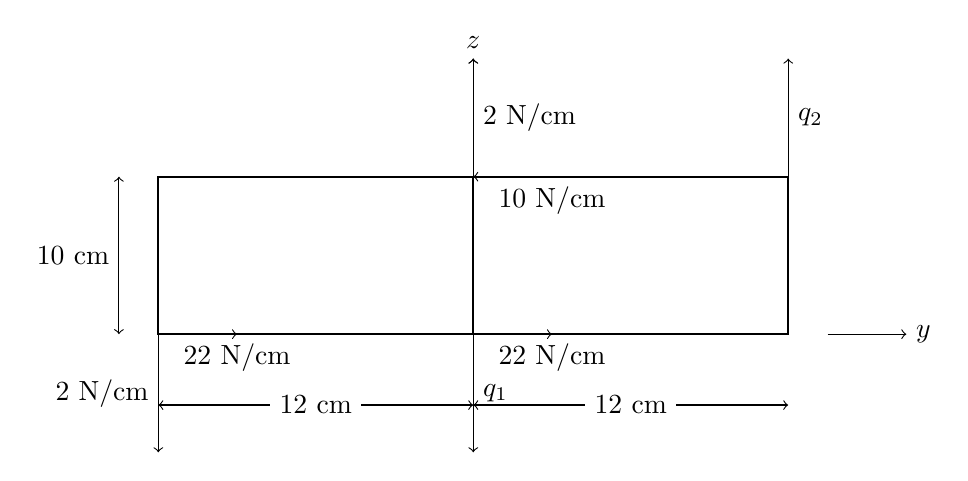
\begin{tikzpicture}


    % Define coordinates for the points
    \coordinate (A) at (0,0);
    \coordinate (B) at (4,0);
    \coordinate (C) at (4,2);
    \coordinate (D) at (0,2);
    \coordinate (E) at (8,0);
    \coordinate (F) at (8,2);

    % Draw the rectangles (two boxes)
    \draw[thick] (A) -- (B) -- (C) -- (D) -- cycle; % Left rectangle
    \draw[thick] (B) -- (E) -- (F) -- (C);          % Right rectangle

    % External force arrows
    \draw[->] (A) -- ++(0,-1.5) node[midway, left] {2 N/cm};  % Bottom left vertical force (2 N/cm)
    \draw[->] (C) -- ++(0,1.5) node[midway, right] {2 N/cm};  % Top left vertical force (2 N/cm)
    \draw[->] (F) -- ++(0,1.5) node[midway, right] {$q_2$};   % Top right unknown force (q2)
    
    % Horizontal force arrows at the bottom
    \draw[->] (A) -- ++(1,0) node[below] {22 N/cm};   % Bottom left horizontal force (22 N/cm)
    \draw[->] (B) -- ++(1,0) node[below] {22 N/cm};   % Bottom right horizontal force (22 N/cm)
    
    % Internal horizontal force between rectangles
    \draw[<-] (C) -- ++(1,0) node[below] {10 N/cm};   % Internal horizontal force (10 N/cm)

    % Vertical force at the right-bottom (q1)
    \draw[->] (B) -- ++(0,-1.5) node[midway, right] {$q_1$};  % Bottom right unknown force (q1)

    % Dimensions
    \draw[<->] (A) ++(0,-0.9) -- ++(4,0) node[midway, fill=white] {12 cm};   % Bottom left length (12 cm)
    \draw[<->] (B) ++(0,-0.9) -- ++(4,0) node[midway, fill=white] {12 cm};   % Bottom right length (12 cm)
    \draw[<->] (D) ++(-0.5,0) -- ++(0,-2) node[midway, left, fill=white] {10 cm};   % Left height (10 cm)

    % Axes
    \draw[->] (8.5,0) -- ++(1,0) node[right] {$y$};   % y-axis
    \draw[->] (4,2.5) -- ++(0,1) node[above] {$z$};   % z-axis



\end{tikzpicture}
\end{document}
